\chapter{Introduction}

\section{The Rising of Hardware Acceleration}

With the end of Dennard Scaling~\cite{dennard}, the amount of performance one can extract from a CPU is reaching a limit.
To provide general-purpose flexibility, CPUs spend the majority of resources and energy on overheads, 
including dynamic-instruction fetching and scheduling, branch prediction, and a cache hierarchy, etc., 
with less than 20\% of 
the energy on the actual computation~\cite{mark}.
Even worse, power wall is limiting the entire multicore family
to reach the doubled performance per generation scaling enabled by technology scaling in the 
past~\cite{multicorescale}.

For this reason, hardware acceleration is emerging in various compute-intensive application domains 
to provide orders of magnitude acceleration, enabling algorithms that were otherwise
infeasible~\cite{genomicaccel, bioaccel, fpgadeeplearn, fpgacripto}.
Examples include widely adopted General-Purpose Graphics Processing Units (GPGPUs) 
in computational genomics, signal processing, and
deep learning, graph processing~\cite{genomicaccel, bioaccel, fpgacloudsurvey}.
Moreover, many recent efforts are spent on leveraging application domain knowledge in hardware design to enable 
continued performance scaling while meeting the power budget~\cite{turinglecture}.
As artificial intelligence receiving great success in industry and business,
recent years have seen a growing interest in machine learning accelerators;
these accelerators contain specialized circuits for ML kernels that dramatically improve the compute
efficiency~\cite{dadiannao,tpu,eie,chen2017eyeriss,tangram,truenorth}.

Nonetheless, it is non-trivial to achieve good utilization with these accelerators.
While the peak FLOPS of GPU has increased by over 20x in the past 10 years, the achievable FLOPS is
not increasing accordingly~\cite{floptrend, gpuperfana}.
The massive threads in GPU require embarrassedly parallel workloads to fully saturate the compute
throughput. GPU's bulk-synchronous nature also causes poor cache efficiency; data are spilled
off-chip before getting reused~\cite{gpuinefficiency}.
On the outer hand, 
while extremely efficient for certain models, machine learning accelerators are highly
specialized for specific kernels, especially general matrix multiply (GEMM) and convolution.
However, ML algorithms evolve much faster than the development and manufacture cycle of hardware, 
leading to inefficiency or even unsupported applications.
For example, hybrid models, such as Mask R-CNN~\cite{maskrcnn} and DeepLab~\cite{deeplab}, contain
combinations of GEMM-compatible and incompatible operations, both computationally expensive.
Fixed-functional accelerators focusing on GEMM operations, such as TPU~\cite{tpu}, 
have to rely on CPUs for unsupported operations or
convert non-GEMM operations to GEMM operations, resulting in a large performance gap between the
peak and effective FLOPS~\cite{effflexdnnaccel}.
\Cref{fig:peakutil} illustrates a trade-off between average utilization of the peak FLOPS over a range
of applications and the peak FLOPS available on the hardware.

\begin{figure*}
\centering
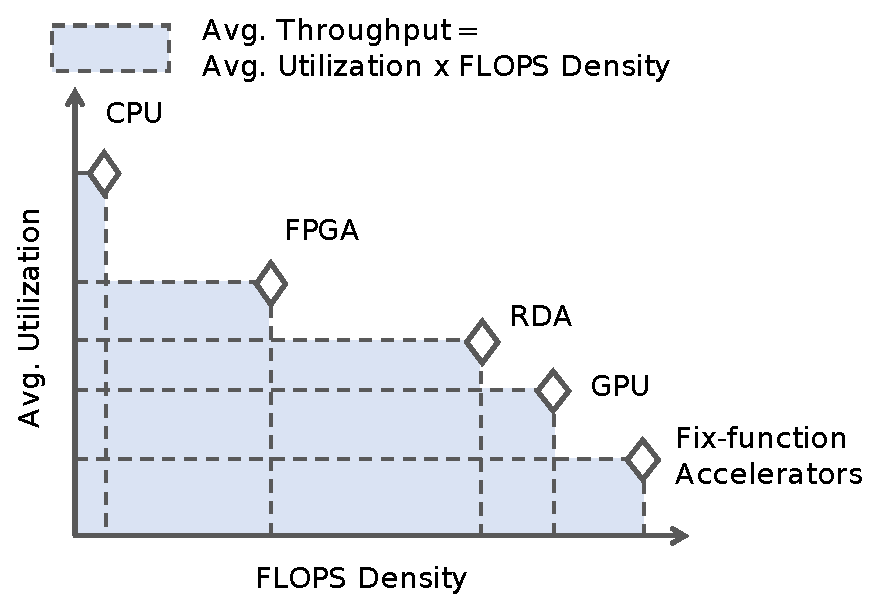
\includegraphics[width=0.4\textwidth]{figs/peakutil.pdf}
\caption[Average utilization vs. peak compute density trade-off]{
 Tradeoff between the average utilization of the peak FLOPS over a range of applications vs. the peak compute density 
 among different architectures.
 The shaded area indicates the effective FLOPS achieved.
 With all the dynamic scheduling hardware in CPUs, such as prefetching and branch prediction, 
 CPUs can achieve a fairly decent instruction per cycle (IPC) for data-analytic workloads that have a 
 regular control flow. 
 However, overheads to support flexibility, security, and programmability in CPUs result in a low FLOPS
 density. 
 While GPU and fix-function accelerators have a high FLOPS density, they are prone to
 underutilization due to variation in application characteristics. 
 Fine-grained reconfigurable datapath makes it easy to utilize on-chip resources of an FPGA.
 However, the soft logics and overheads in routing resources lead to a low resource density and clock frequency.
 RDAs have the right balance between flexibility and efficiency, which gives a good overall average utilization.
}
\label{fig:peakutil}
\end{figure*}

Reconfigurable spatial architectures overcome this limitation by changing their datapaths based on
an application's need.
Applications are configured at the circuit-level without dynamic instruction fetching and scheduling,
hence improving energy-efficiency~\cite{calhoun,fpgaPower}.
In addition to instruction, data, and task-level parallelism exploited by processor architectures,
spatial architectures also exploit instruction and task-level pipelining that further increases the compute throughput~\cite{spatial-computation}.
Exploiting pipeline parallelism enables spatial architectures to achieve high-throughput
without massively parallelizing every stage of the program.
Flexible datapath also permits resource distribution proportional to the compute intensity of
program stages.
A key performance optimization on reconfigurable accelerators is an application-level design space
exploration 
searching for the best resource distribution scheme that balances the compute pipeline~\cite{dse_koeplinger}.

One of the mainstream reconfigurable spatial architecture is 
Field Programmable Gate Arrays (FPGAs) that support fine-grain, 
bit-level reconfigurability with a soft logic fabric~\cite{fpga-survey}.
The flexible interconnect and lookup table-based logic gate can be configured to implement arbitrary
datapaths.
FPGAs have been used to deploy services commercially~\cite{microsoft, baidu, deephi} and can be rented on the AWS F1 cloud~\cite{aws}. 
Although they have been around for a long time, FPGAs are not broadly accepted among high-level
application programmers due to their low-level programming interface and long compilation times.
Fine-tuning applications on FPGAs requires expertise in digital design and takes a long development cycle, which hinder their accessibility to the general software community.
As application-level accelerators, FPGAs also suffer from overhead in fine-grained reconfigurability; 
studies have shown that over 60\% of the chip area of an FPGA is spent on routing resources~\cite{fpgaSurvey, calhoun, fpgaPower}. 

%Lately, Reconfigurable Dataflow Architecture (RDAs)~\cite{plasticine, ti, streamdataflow,neuflow,cnndataflow,dataflowarch} are emerging as a new class of spatial accelerators that 
%retain the desired level of flexibility and energy efficiency without 
%the area overhead and low clock frequency due to bit-level reconfigurability.
%As a subclass of Coarse-Grained Reconfigurable Arrays (CGRAs), RDAs also have
%coarse-grained building blocks, such as ALUs, register files, and memory controllers, 
%distributed in a programmable, word or vector-level static interconnect~\cite{adres, kress, dyser, 
%piperench, tartan, hrl, hycube}.

In contrast to fine-grained reconfigurable architectures,
Coarse-Grained Reconfigurable Arrays (CGRAs) are spatial architectures with 
coarse-grained building blocks, such as ALUs, register files, and memory controllers, 
distributed in a programmable, word or vector-level static interconnect~\cite{adres, kress, dyser, piperench, tartan, 
hrl, hycube}.
We refer a subclass of CGRAs with dataflow-driven execution model as Reconfigurable Dataflow
Architectures (RDAs)\footnote{Dataflow overlay architectures on FPGA are technically also RDAs, which are not the primary concern in the discussion of this work.}~\cite{plasticine, ti, streamdataflow,neuflow,cnndataflow,dataflowarch}.
Lately, RDAs are emerging as a new class of spatial accelerators that retain the desired level of
flexibility and energy efficiency without the area overhead and low clock frequency of bit-level reconfigurability.
Our previously proposed RDA--Plasticine--has demonstrated a promising acceleration of dense, sparse, database, and streaming applications~~\cite{plasticine, gorgon, multijoin,prabhakarthesis}.
To meet the computing demand of recent data-analytic workload, Plasticine is a large-scale RDA
compared to traditional CGRAs. 
\Cref{tab:ops} shows the OPS comparison across a few CGRAs proposed in the prior works.

\begin{table}
  \centering
\begin{tabular*}{0.88\textwidth}{cccccc}
  \toprule
  \textbf{Architectures} & DySER~\cite{dyser} & TI~\cite{ti} & REVEL~\cite{revel}
  & Plasticine~\cite{plasticine} & Gorgon~\cite{gorgon}\\\midrule
  \textbf{OPS} & 128GOPS & 64GOPS & 300GOPS & 12.3TFLOPS & 38.4TFLOPS \\
  \bottomrule
\end{tabular*}
\caption[OPS comparison of different CGRAs]{OPS comparison of different CGRAs. Gorgon is a
Plasticine variant proposed for joint machine learning and database acceleration.}
\label{tab:ops}
\end{table}

The scale of Plasticine introduces challenges in network-on-chip design to sustain 
bandwidth requirements while staying energy-efficient.
The compilation strategy also needs to explore multiple-levels of
concurrency in the program to saturate the compute throughput of a large-scale RDA;
this strategy must introduce minimum synchronization overhead to maximize the scalability of the
mapped designs.

\section{The Need for Flexible Interconnects}
Applications are mapped to RDAs by distributing computations spatially across multiple processing
blocks and executing them in a pipelined, data-driven fashion. 
In traditional Networks-on-Chip
(NoCs) for multicore systems, communication is the result of explicit message passing between
parallel workers or cache misses that generate messages for coherence protocol; this traffic is bursty and
relatively infrequent. 
On RDAs, however, applications are distributed by parallelizing and pipelining; 
pipelining introduces frequent and throughput-sensitive communication. 
Applications with different characteristics, such as compute vs. memory-bound, also exhibit 
very different communication patterns.

\begin{figure*}
\centering
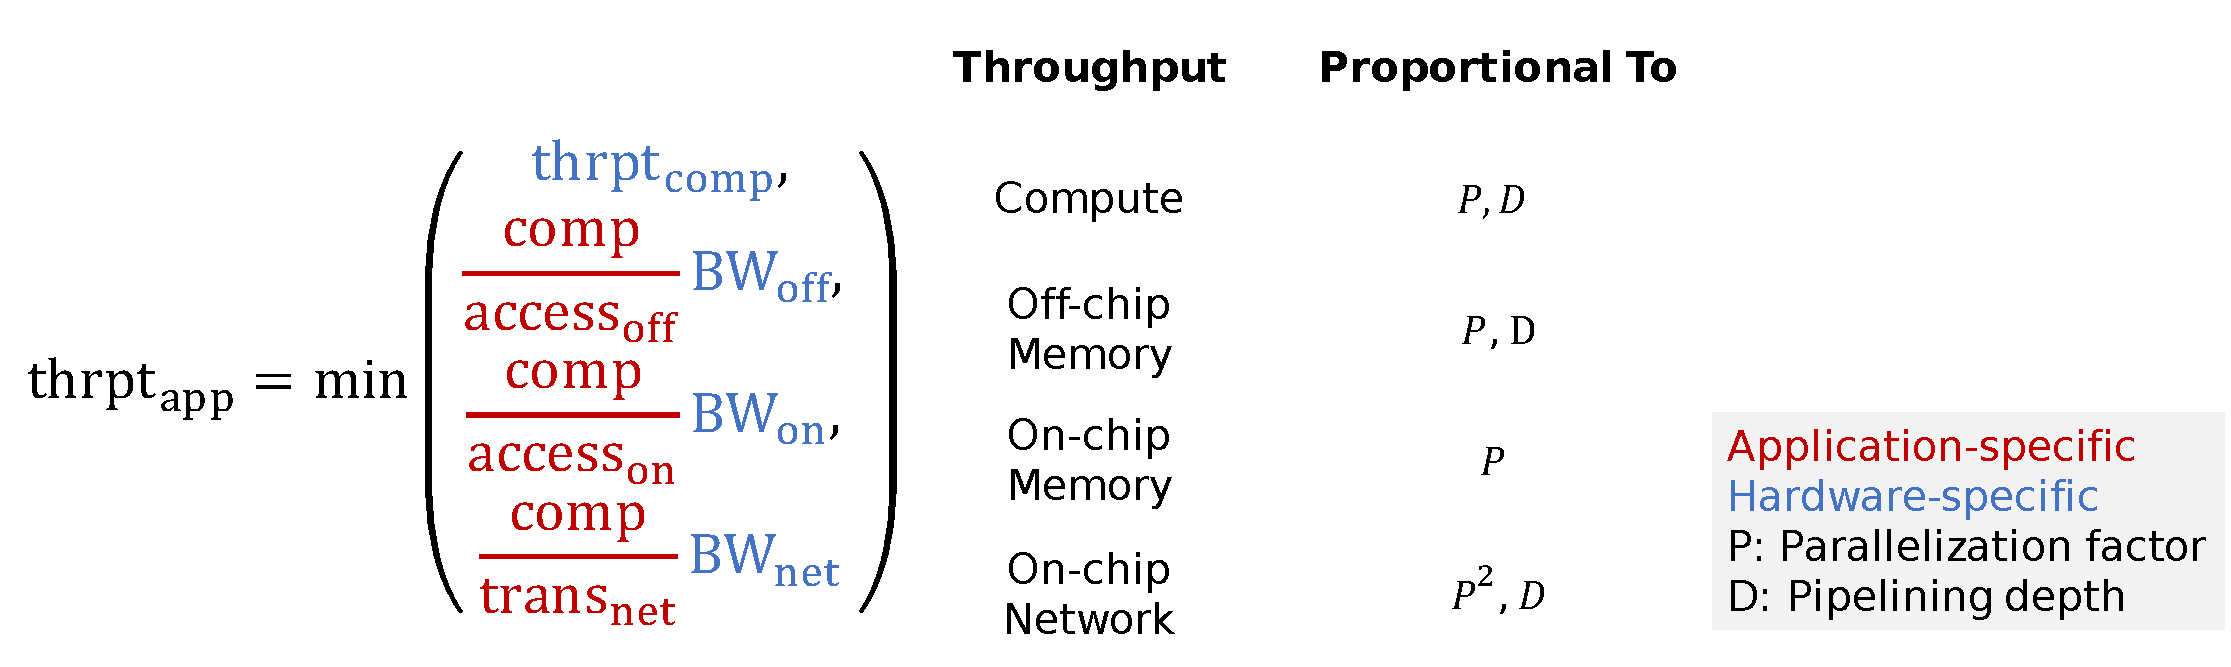
\includegraphics[width=1\textwidth]{figs/perfmodel.pdf}
\caption[High-level performance model of a spatial architecture]{
High-level performance model of a spatial architecture. 
}
\label{fig:perfmodel}
\end{figure*}

\Cref{fig:perfmodel} shows a high-level performance model of a spatially pipelined and parallelized
reconfigurable architecture.
Due to pipelined execution, the performance of a spatial architecture is mainly determined by throughput as
supposed to latency. 
Compute, on and off-chip memory accesses, and network become an integrated pipeline;
overall performance is limited by the pipeline stage with the lowest throughput.
The red terms in the equation are application-specific and capture the compute, memory, or IO-bound characteristics.
The blue terms are the bandwidth and FLOPS available on the hardware.
While the compute and memory access in application increases linearly with parallelization factor and pipelining depth,
the required network bandwidth from the applications increases quadratically with increasing parallelism.
This means as we going to larger chip size, the network bandwidth must grow super linearly to achieve a perfect performance scaling, unless exploring pipeline parallelism.

RDAs need the right amount of interconnect flexibility to achieve good resource utilization; 
an inflexible interconnect constrains the space of
valid application mappings and hinders resource utilization. 
Furthermore, 
in the quest to increase compute density, RDA datapaths now 
contain increasingly coarse-grained processing blocks such as pipelined, vectorized functional 
units~\cite{plasticine, piperench, xilinx-acap}.
Plasticine, as an example, has a 512-bit vector bus, which necessitates coarser communication and higher on-chip interconnect bandwidth to avoid creating performance bottlenecks. 
Although many hardware accelerators with large, vectorized datapaths have fixed local networks~\cite{brainwave}, there is a need for more
flexible global networks to adapt to future applications.
Consequently, interconnect design for these RDAs involves achieving a balance between the often conflicting requirements of high bandwidth and high flexibility.

\section{The Gap between High-Level DSLs and Dataflow Accelerators}

Recent years have seen an explosion of hardware accelerators, primarily motivated by AI
applications~\cite{tangram,truenorth,memristive,dadiannao,pudiannao,chen2017eyeriss,eie,reno,convengine,minerva,dnpu,cbrain}. 
Research in software infrastructures for these accelerators, however, is just emerging.
Unlike CPUs, accelerators do not support a standard instruction set architecture (ISA), alleviating the overhead from
layers of abstractions and the burden of backward compatibility. 
Nonetheless, lack of a common abstraction makes it very hard to share compiler infrastructure
across accelerators. 

Most RDAs comes with a co-designed software layer that is very low-level and restrictive,
requiring expert knowledge in hardware architecture to efficiently target the accelerator.
On the other side,
machine learning frameworks~\cite{tensorflow,caffe,pytorch,taco,onnc,tc} provide high-level and 
succinct front-end abstraction that targets multiple hardware platforms. 
Yet most of theses frameworks only target mainstream accelerators, such as GPUs and FPGAs.
Very few of the accelerators mentioned above can support more than a few proof-of-concept models
with an end-to-end integration with these frameworks.

\begin{figure*}
\centering
\begin{subfigure}[b]{0.48\textwidth}
\centering
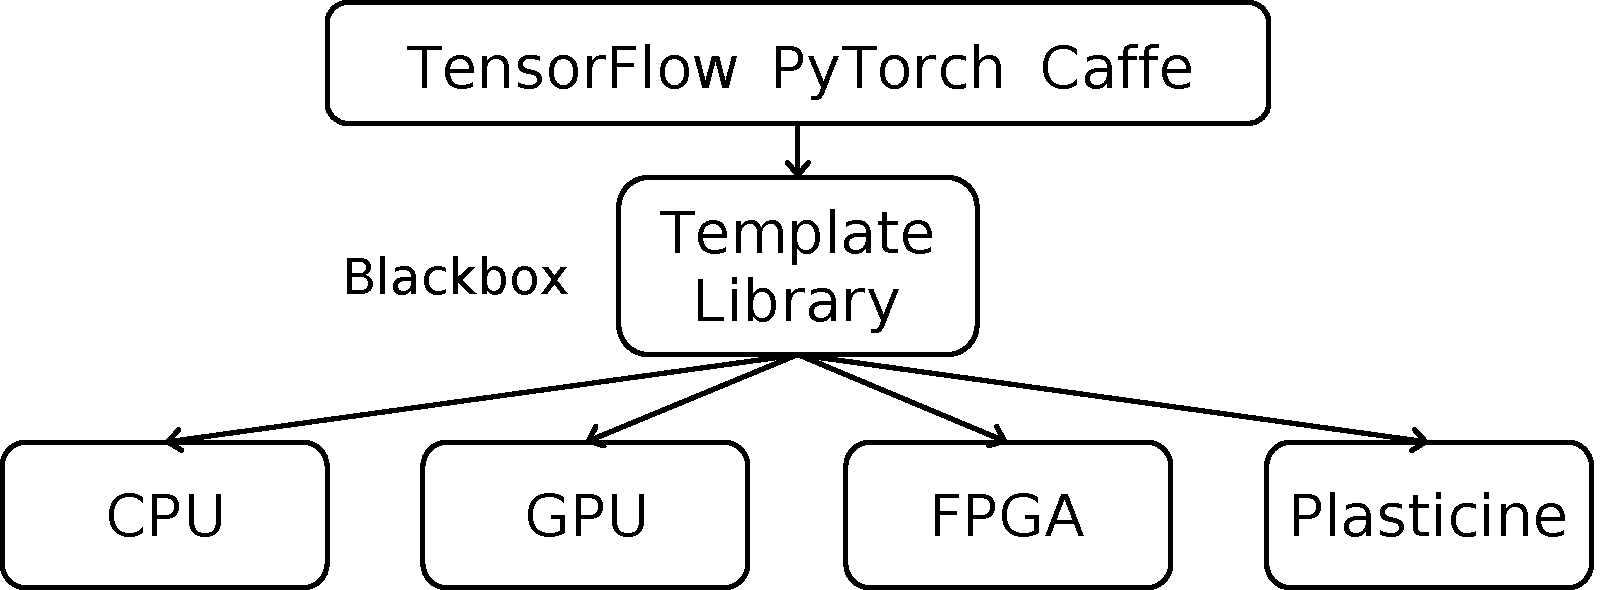
\includegraphics[width=1\textwidth]{figs/blackbox.pdf}
\caption{
  Blackbox approach in~\cite{tensorflow,pytorch,caffe}.
}
\end{subfigure}
\hfill
\begin{subfigure}[b]{0.48\textwidth}
\centering
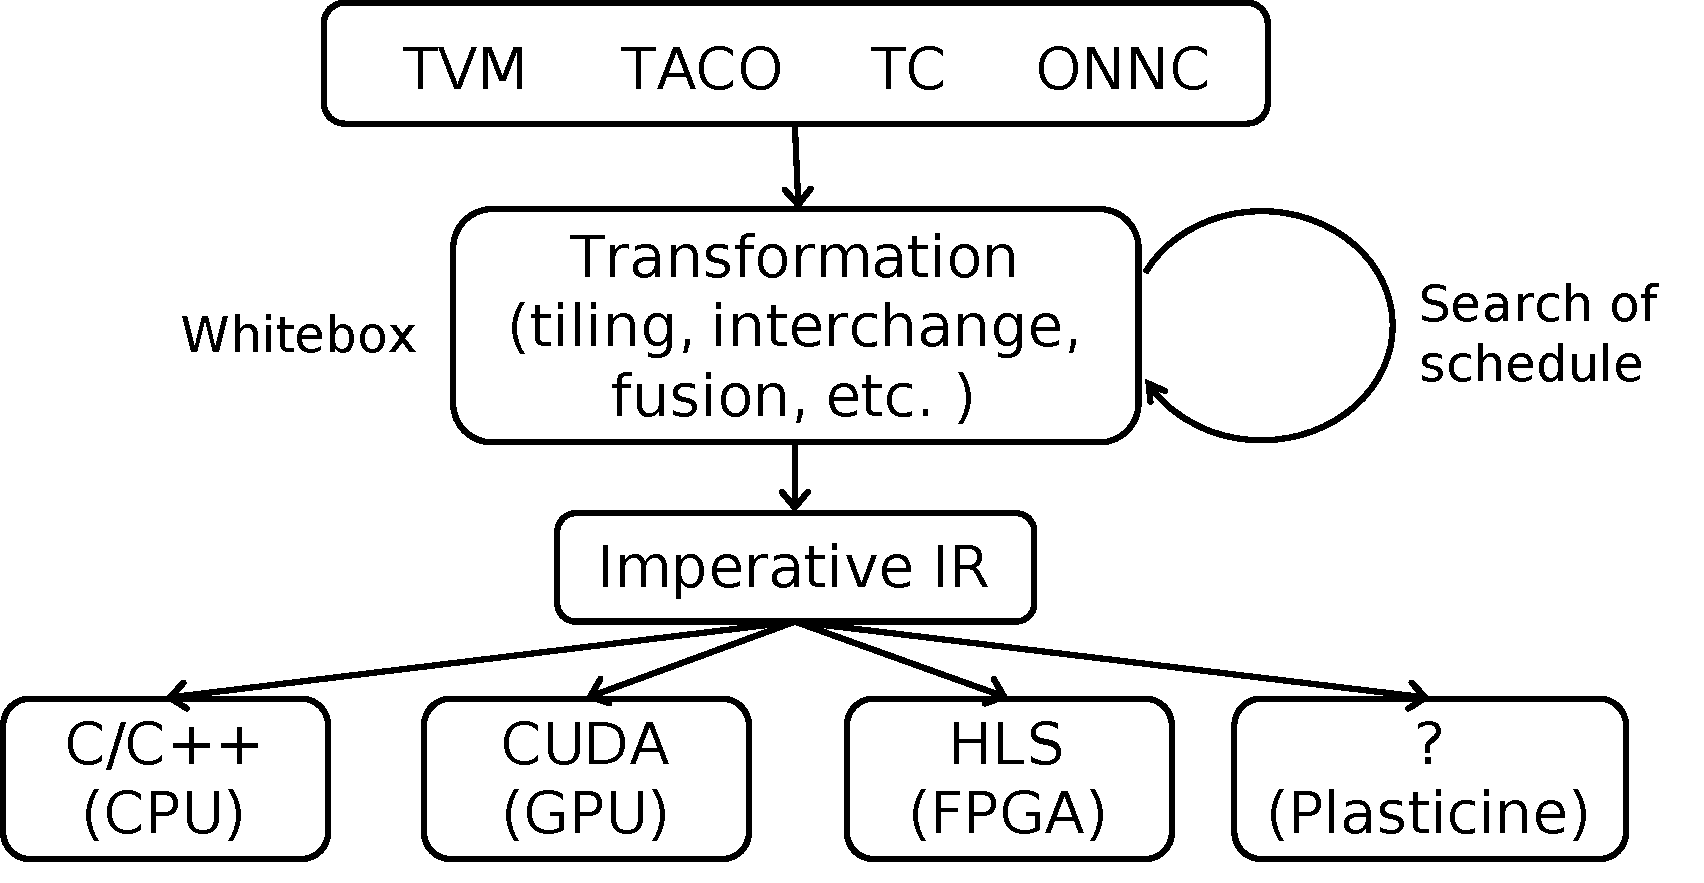
\includegraphics[width=1\textwidth]{figs/whitebox.pdf}
\caption{
  Whitebox approach in~\cite{tvm,taco,tc,onnc,halide}.
}
\end{subfigure}
\caption[Big picture of machine learning frameworks]{
  Big picture of machine learning frameworks.
}
\label{fig:bigpic}
\end{figure*}

Part of the reason behind this is the massive engineering effort to program these accelerators.
Frameworks like TensorFlow~\cite{tensorflow} and PyTorch~\cite{caffe} uses a template library
approach, as shown in ~\Cref{fig:bigpic} (a).
These frameworks treat operations in the ML dataflow graph as black-box kernels and implement
every operation for every backend, requiring expensive engineering hours and hardware expertise to
fine-tune each accelerator.
Furthermore, cross-kernel optimizations, such as fusion, often provide orders of magnitude improvement in efficiency.
%%TODO: citation
Recent studies in sparse ML also show promising speedup on large ML models~\cite{eie}. 
However, sparse kernels require various data formats with very different implementation than the dense
version~\cite{tacosparse}.
In the black-box approach, each fused operation and data format corresponds to a new black-box
kernel.
As a result, the combination of required templates easily becomes untractable.

The alternative white-box approach showing in~\Cref{fig:bigpic} (b) uses a succinct front-end
representation, such as index notations~\cite{taco}, to express the computation of a kernel.
This representation, however, cannot be directly mapped to accelerators due to various physical
constraints.
The framework then uses a series of transformations and optimizations to reformulate the kernel to an imperative implementation that can be supported by the accelerator. 
The transformation is often target-specific and studies have demonstrated ML-based cost models to
facilitate the automatic searching of backend-specific schedules~\cite{tvm}.
Next, the compiler can easily translate the imperative intermediate representation (IR) to the imperative front-ends of different
accelerators.

To enable easy integration of the white-box approach, we introduce a compiler--\name--that raise
the programming abstraction of Plasticine to an imperative, loop-based
language for general reconfigurable hardware---Spatial~\cite{spatial}.
Plasticine is a pure dataflow accelerator without a centralized scheduler that
executes instructions. This design makes the architecture very scalable to achieve FLOPS comparable
to high-end GPUs and FPGAs.
Nonetheless, it is not intuitive nor easy to implement a linear algebra kernel with the low-level
declarative streaming configurations.
By support imperative constructs on a data-flow architecture efficiently, \name not only improves
the programmability of Plasticine, but also enables cross kernel optimizations.
These optimizations have demonstrated an average 30x speedup over a Tesla V100 GPU and 2x speedup over
a Stratix 10 FPGA with a Plasticine chip with much less on-chip resource than the baseline architectures~\cite{tz_rnn}.

\section{Contribution}

This thesis work builds upon the prior work on the Plasticine architecture~\cite{plasticine} and the Spatial
compiler~\cite{spatial}.
We address the programmability and scalability challenges from a software
and a hardware perspective.
We first introduce the Plasticine compiler---\name---that maps Spatial applications to Plasticine.
Next, we present several architectural augmentations to Plasticine to increase the flexibility in interconnect, memory access patterns, and control flow.

The key contributions of this work are summarized below:
\begin{enumerate}
    \item We propose an imperative to dataflow transformation that implements imperative control constructs, such as nested loops and branch statements, on a pure dataflow architecture.
      This mapping strategy introduces minimum point-to-point synchronization that efficiently scales performance over distributed on-chip resources.
    \item We introduce compiler-enforced memory consistency to preserve memory ordering in the imperative program between distributed memory accesses.
    \item We illustrate a systematic approach to address physical constraints in a hierarchical RDA.
      We evaluate the tradeoff between a traversal-based vs. solver-based algorithms for program partitioning. 
      %We also present how to efficiently partition a logical memory over distributed
      %scratchpads.
    \item We use resource virtualization and optimizations to minimize fragmentation in resource allocation with heterogeneous compute tiles.
    \item We demonstrate an evaluation of the scalability of \name and effectiveness of compiler optimizations.
      We show a 1.9x average speedup over a Tesla V100 with a Plasticine with 8x less in on-chip
      resources due to the efficient use of the accelerator.
    \item We analyze the key communication patterns exhibited by spatial architectures by characterizing a variety of benchmarks from different domains.
    \item We demonstrate that static compiler knowledge can be used to reduce routing congestion.
    \item We give a comprehensive quantitative analysis of the performance, area, and energy trade-offs 
      involved in choosing an RDA network, using a cycle-accurate simulator and ASIC synthesis with a \SI{28}{nm} industrial technology library.
      We explore a variety of design points, including static, dynamic, and hybrid networks, decreased flit widths and VC counts for dynamic networks and different flow-control strategies for static networks.
    \item We show that bandwidth is the most critical metric to assess network performance for RDA,
      due to their pipelined execution nature. We found static-dynamic hybrid networks can give
      better energy efficiency by reducing overprovisioning in purely static networks and reducing
      data movement.
    \item We present changes in Plasticine required to support flexible memory access patterns and flexible control flow.
\end{enumerate}

%In this work, we start by detailing the key considerations involved in building an RDA network, including those arising from network design, RDA architecture, and the characteristics of spatially mapped applications.
%Network designs must be carefully considered because vectorization magnifies inefficiencies: the increased network area of a vectorized design ensures that any overhead has a significant impact.
%Next, we evaluate the performance, area, and power requirements of several interconnection designs using cycle-accurate simulation and ASIC synthesis of a switch and router with a \SI{28}{nm} industrial technology library.
%We then explore a variety of design points, including static, dynamic, and hybrid networks, decreased flit widths and VC counts for dynamic networks and different flow-control strategies for static networks.

%We show that RDA network designs must consider application characteristics and the execution model of the underlying architecture.
%Performance scales strongly with network bandwidth, with an 8x average performance gap between the best and worst configurations. 
%The hybrid network gives the best network energy-efficiency: a 1.83x average improvement over the static network. On pipelined architectures,
%hybrid networks can also match the performance per area of higher bandwidth, purely static networks with less than 8\% performance loss.

\section{Outline}
The rest of this thesis is organized as follow:
\Cref{sec:background} gives a background on the execution schedule of spatial
architectures, the front-end imperative language of \name compiler, and the targeting architecture--Plasticine.
\Cref{sec:compiler} goes over the \name compiler.
\Cref{sec:arch} details the augmentations to the Plasticine architectures and the
Network-on-chip study.
\Cref{sec:related} summarizes the related work.
\Cref{sec:conclusion} concludes our work.
